\documentclass[../piano-di-progetto.tex]{subfiles}
\begin{document}

\subsection{Completamento di dettaglio}
In questo macro-periodo verranno progettate e implementate tutte le restanti funzionalità richieste, ottenendo un prodotto completo. Verranno svolti cinque incrementi.
\subsubsection{Ruoli}
Durante i successivi cinque incrementi, viene richiesta la presenza dei seguenti ruoli:
\begin{itemize}
    \item Responsabile;
    \item Amministratore;
    \item Progettista;
    \item Verificatore.
\end{itemize}

%\subsubsection{Attività}
%Per semplicità, questa macro viene suddivisa in periodi:
%%
%\begin{itemize}
%    \item \textbf{I periodo (2020-05-18 2020-06-10)}: vengono %effettuati cinque incrementi per la realizzazione di una %\glossario{product baseline}, verranno illustrati nella prossima %sottosezione;
 %   \item \textbf{II periodo (2020-06-11 2020-06-17)}:
 %       \begin{itemize}
 %           \item Preparazione della presentazione;
 %           \item Verifica.
 %       \end{itemize}
%\end{itemize}


\subsubsection{V incremento}

 Vengono stabiliti i seguenti obiettivi per il quinto incremento:
 \begin{itemize}
     \item Implementazione dell'algoritmo di SVM per la generazione dei predittori nel programma di addestramento;
     \item Integrazione dell'algoritmo con il resto dei componenti.
 \end{itemize}

\paragraph{Attività}
Le attività verranno svolte in un unico periodo:
\\
\\
\textbf{Periodo unico (2020-05-11 - 2020-05-15):}
\begin{itemize}
    \item Progettazione;
    \item Codifica: implementazione delle funzionalità progettate;
    \item Preparazione della presentazione per RQ;
    \item Verifica: controllo delle funzionalità implementate.
\end{itemize}

\subsubsection{VI incremento}

 Vengono stabiliti i seguenti obiettivi per il sesto incremento:
 \begin{itemize}
     \item Implementazione del caricamento dei predittori nel plug-in;
     \item Implementazione della possibilità di scegliere nel plug-in i nodi su cui effettuare predizioni.
 \end{itemize}

\paragraph{Attività}
Le attività verranno svolte in un unico periodo:
\\
\\
\textbf{Periodo unico (2020-05-16 - 2020-05-21):}
\begin{itemize}
    \item Progettazione;
    \item Codifica: implementazione delle funzionalità progettate;
    \item Stesura del manuale;
    \item Verifica: controllo delle funzionalità implementate e dei documenti modificati.
\end{itemize}


\subsubsection{VII incremento}
 Vengono stabiliti i seguenti obiettivi per il settimo incremento:
 \begin{itemize}
    \item Implementazione delle predizioni del plug-in;
    \item Implementazione del collegamento tra predizioni e front-end.

\end{itemize}
\paragraph{Attività}
Le attività verranno svolte in un unico periodo:
\\
\\
\textbf{Periodo unico (2020-05-22 - 2020-05-28):}
\begin{itemize}
    \item Progettazione;
    \item Codifica: implementazione delle funzionalità progettate;
    \item Stesura del manuale;
    \item Verifica: controllo delle funzionalità implementate e dei documenti modificati.
\end{itemize}


\subsubsection{VIII incremento}

 Vengono stabiliti i seguenti obiettivi per l'ottavo incremento:
 \begin{itemize}
    \item Implementazione della gestione degli errori;
    \item Implementazione delle impostazioni per la rimozione del plug-in;

 \end{itemize}
\paragraph{Attività}
Le attività verranno svolte in un unico periodo:
\\
\\
\textbf{Periodo unico (2020-05-29 - 2020-06-03):}
\begin{itemize}
    \item Progettazione;
    \item Codifica: implementazione delle funzionalità progettate;
    \item Stesura del manuale;
    \item Verifica: controllo delle funzionalità implementate e dei documenti modificati.
\end{itemize}


\subsubsection{IX incremento}

 Vengono stabiliti i seguenti obiettivi per l'incremento:
 \begin{itemize}
    \item Implementazione delle impostazione degli alert;
    \item Implementazione della possibilità di applicare la trasformazione logaritmica nel programma di addestramento;
    \item Implementazione della possibilità di applicare la trasformazione esponenziale nel programma di addestramento.

 \end{itemize}

\paragraph{Attività}
Le attività verranno svolte in un unico periodo:
\\
\\
\textbf{Periodo unico (2020-06-04 - 2020-06-10):}
\begin{itemize}
    \item Progettazione;
    \item Codifica: implementazione delle funzionalità progettate;
    \item Stesura del manuale;
    \item Consuntivo di periodo;
    \item Stesura lettera di presentazione;
    \item Verifica: controllo delle funzionalità implementate e dei documenti modificati.
\end{itemize}



\newpage
\begin{landscape}
    \begin{figure}[H]
        \centering
        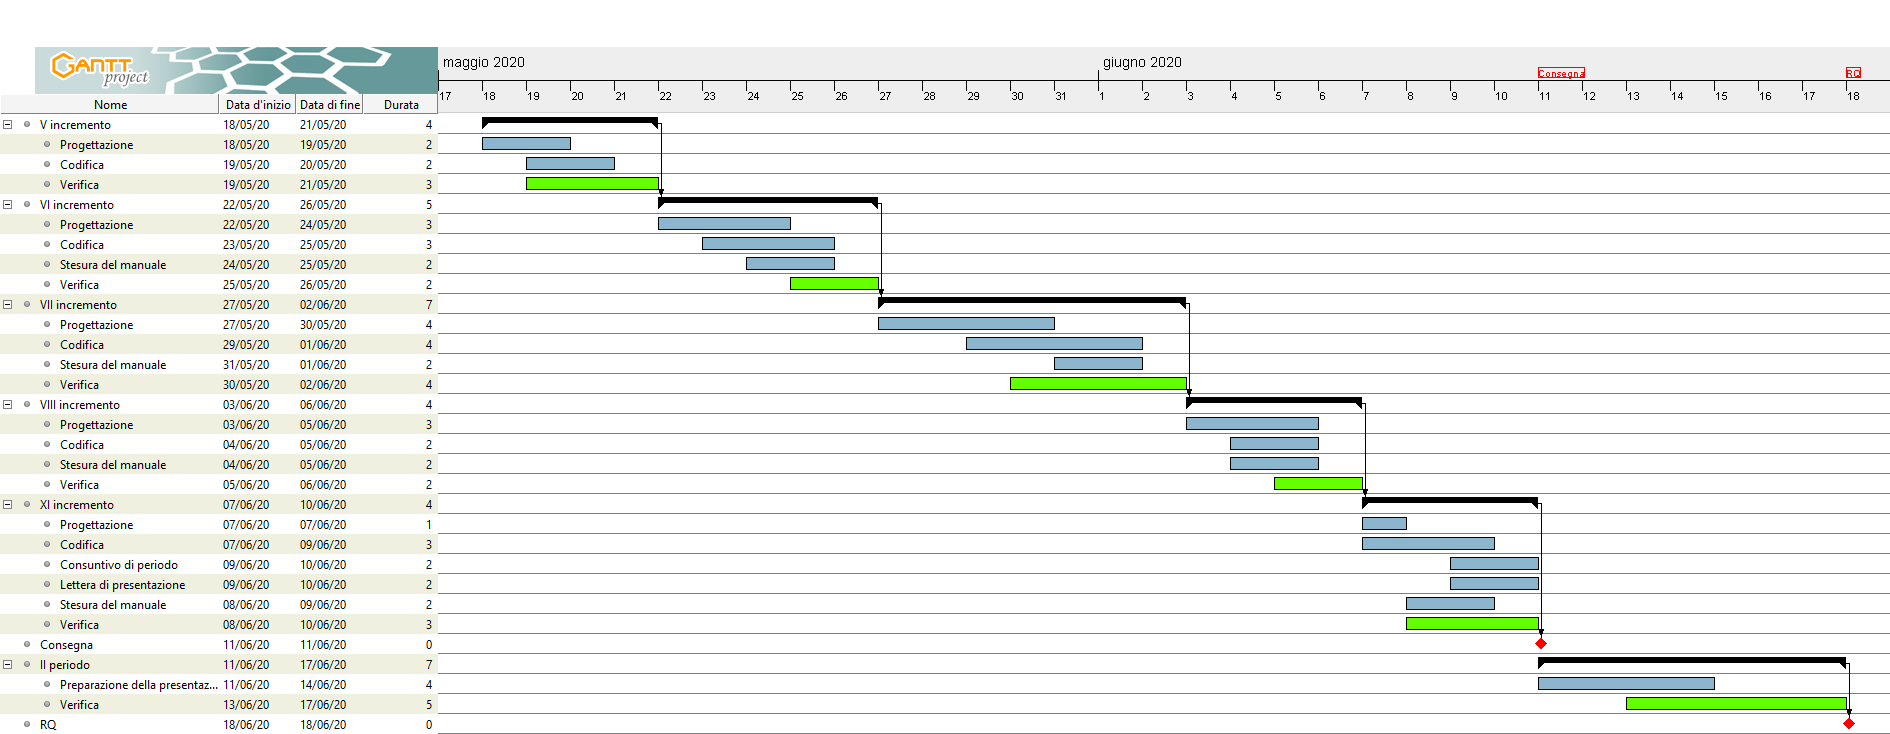
\includegraphics[width=24cm]{img/codifica.png}
        \caption{Diagramma attività nel periodo di codifica di dettaglio}
      \end{figure}
\end{landscape}

\end{document}
